\section{Introduction to Deep Learning} \label{ssec:DL}
Deep Learning is part of the broader framework of Machine Learning and Artificial Intelligence. Indeed all the problems typically faced using ML can also be addressed with DL techniques, for instance, regression, classification, clustering, and segmentation problems. We can think of DL as a universal methodology for iterative function approximation with a great level of complexity. In the last decades, this technology has seen a frenetic diffusion and an incredible development, thanks to the always increasing available computational power, and it has become a staple tool in all sorts of scientific applications.

\subsection{Perceptrons and Multilayer Feedforward Architecture}
Like other artificial learning techniques, DL models aim to \textit{learn} a relationship between some sort of input and a specific kind of output. In other words,  approximating numerically the function that processes the input data and produces the desired response. For example, one could be interested in clustering data in a multidimensional features space, or the detection of objects in a picture, or text manipulation/generation. The function is approximated employing a greatly complex network of simple linear and non-linear mathematical operations arranged in a so-called Neural Network (typically with millions of parameters). The seed idea behind this discipline is to recreate the functioning of actual neurons in the human brain: their entangled connection system and their "ON/OFF" behavior \cite{10.5555/3275328}.

The fondamental unit of a neural network is called perceptron, and it acts as a digital counterpart of a human neuron. As shown in Figure \ref{fig:perceptron} a perceptron collects in input a series on $n$ numerical signals $\vec{x} = 1, x_1, ..., x_n $ and computes a linear wieghted combination with the weights vectors $\vec{w} = w_0, w_1, ..., w_n$, where $w_0$ is a bias factor:

\begin{equation}
    f(\vec{x},\vec{w}) = \chi(\vec{x} \cdot \vec{w}).
\end{equation}

The results of this linear combination are given as input to a non-linear function $\chi(x)$ called the activation function. Typical choices as activation function are any sigmoidal function like $sign(x)$ and $tanh(x)$, but in more advanced applications other functions like ReLU \cite{1803.08375} are used. The resulting function $f(\vec{x},\vec{w})$ has then a simple non linear behaviour. It produces a binary output: 1 if the weighted combination is high enough and 0 if it is low enough, with a smooth modulation in-between the two values.

\begin{figure}
    \centering
    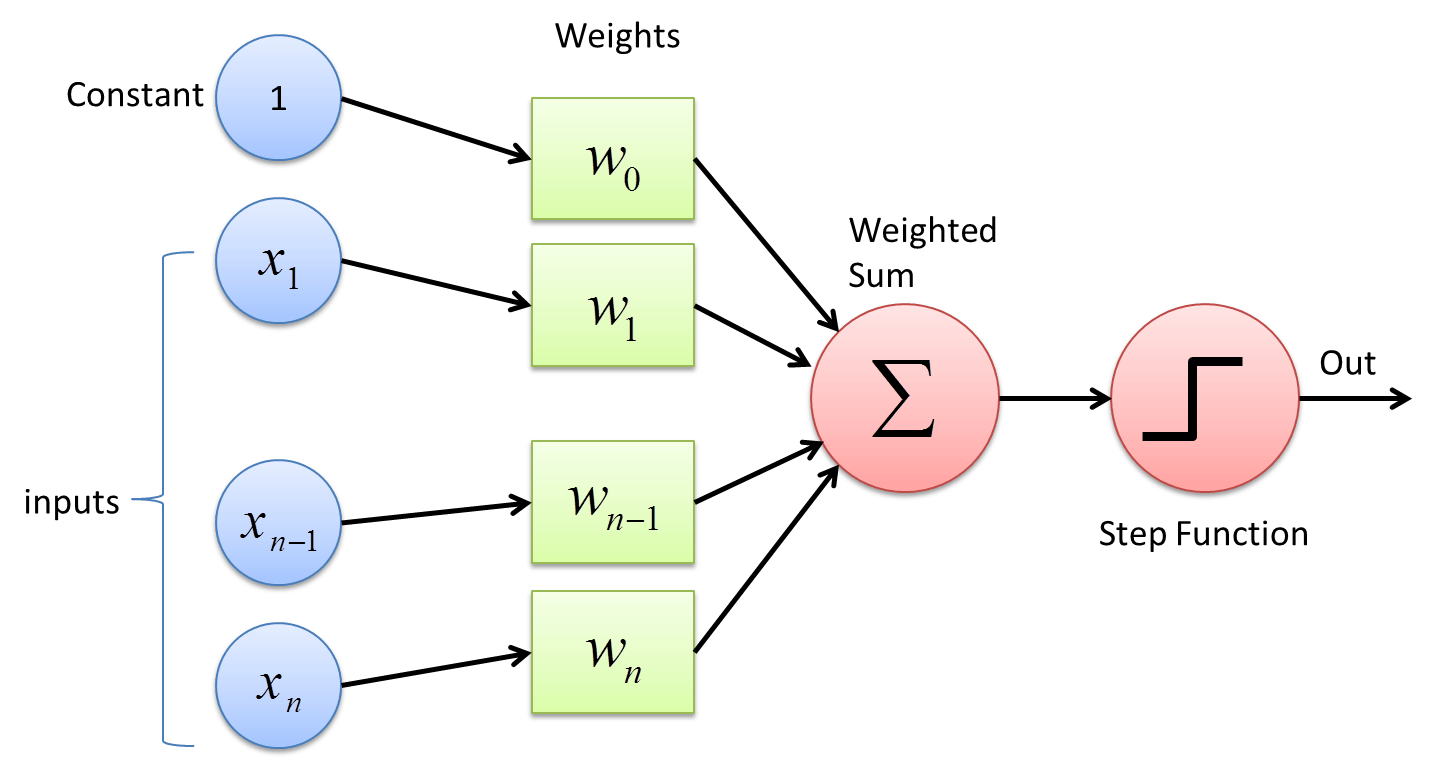
\includegraphics[width = 0.7\textwidth]{images/perceptron}
    \caption{Schematic picture of a single layer perceptron. The input vector is linearly combined with the bias factor and sent to an activation function to produce the numerical "binary" output.}
    \label{fig:perceptron}
\end{figure}

The most common architecture for a NN is the so-called \textit{feed-forward} architecture, where many individual perceptrons are arranged in chained layers, which take as input the output of previous layers along with a straight information flux. More complex architectures could implements also recursive connection, linking a layer to itself, but it should be regarded as sophistication to the standard case. There are endless possibilities of combination and arrangement of neurons inside a NN's layer, but the most simple ones are known as fully-connected layers, where every neuron is linked with each other neuron of the following layer, as shown in Figure \ref{fig:fully_connected}. Each connection has its weight, which contributes to modulate the overall combination of signals. The training of a NN consists then in the adjustment and fine-tuning of all the network's weights and parameters through iterative techniques until the desired precision in the output generation is reached.

\begin{figure}
    \centering
    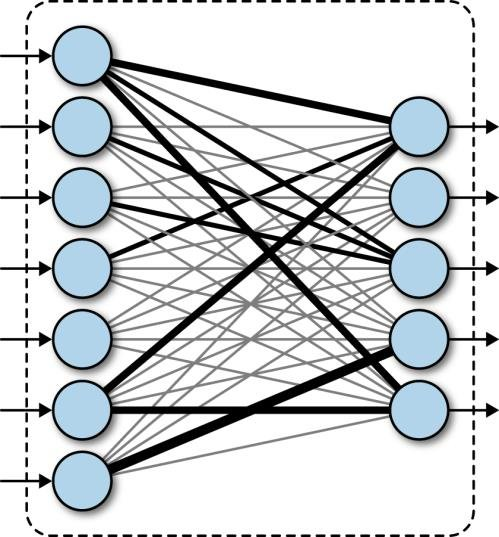
\includegraphics[width = 0.4\textwidth]{images/fully_connected}
    \caption{Schematic representation of a fully connected (or dense) layer. Every neuron from the first layer is connected with every output neuron. The link thickness represent the absolute value of the combination weight for that particular value. }
    \label{fig:fully_connected}
\end{figure}

Although a fully connected network represents the simplest linking choice, the insertion of each weight increases the number of overall parameters, and so the complexity of the model. Thus we want to create links between neurons smartly, rejecting the less useful ones. Depending on the type of data under analysis there are many different established typologies of layers. For example, in the image processing field, the most common choice is the convolutional layer, which implements a sort of discrete convolution on the input data, as shown in Figure \ref{fig:convolutional}. While processing images, the convolution operation confers to the perception of correlation between adjacent pixels of an image and their color channels, allowing a sort of spatial awareness. Furthermore, the majority of traditional computer vision techniques are based on the discrete convolution of images, and on the features extracted from them.

As a matter of principle a NN with just two successive layers, which is called a \textit{shallow} network, and with an arbitrary number of neurons per layer, can approximate arbitrary well any kind of smooth enough function \cite{pinkus_1999}. However, direct experience suggests that networks with multiple layers, called \textit{deep} networks, can reach equivalent results exploiting a lower number of parameters overall. This is the reason why this discipline goes under the name of \textit{deep} learning: it focuses on deep networks with up to tents of hidden layers. Such deep structures allow the computation of what is called deep features, so features of the features of the input data, that allows the network to easily manage concepts that would be bearly understandable for humans.

\begin{figure}
    \centering
    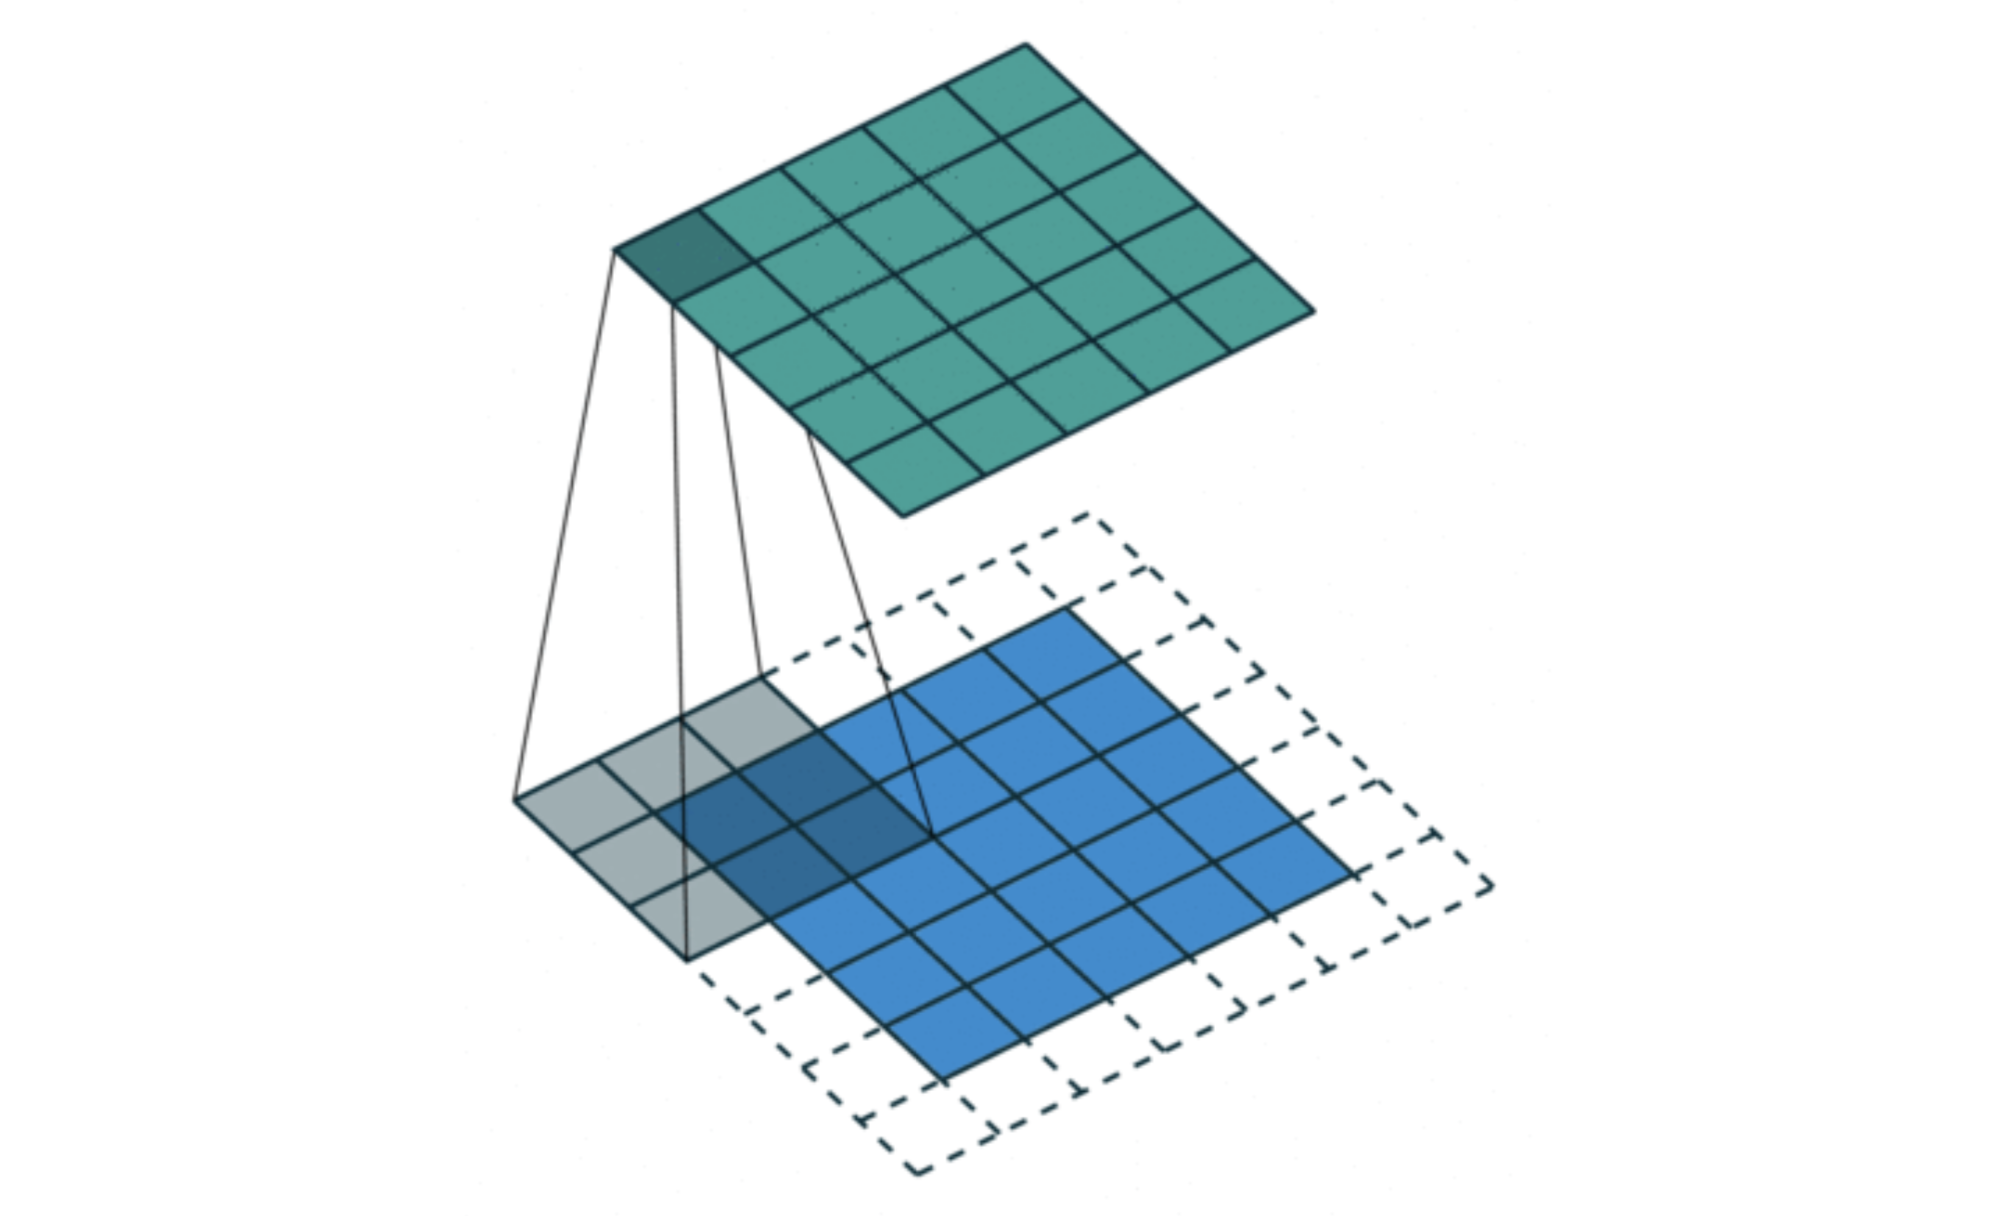
\includegraphics[width = 0.7\textwidth]{images/CL}
    \caption{Schematical representation of a convolutional layer. The input data are processed by a window kernel that slides all over the image. This operation can recreate almost all the traditional computer vision techniques, and can overcome them, creating new operations, which would be unthinkable to hand-engineered.}
    \label{fig:convolutional}
\end{figure}

\subsection{Training of a NN -  Error Back-Propagation}
Depending on the task the NN is designed for, it will have a different architecture and number of parameters. Those parameters are initialized to completely random values, tough. The training process is exactly the process of seeking iteratively the right values to assign to each parameter in the network in order to accomplish the task. The best start to understanding the training procedure is to look at how a supervised problem is solved. In supervised problems, we start with a series of examples of true connections between inputs and correspondent outputs and we try to generalize the rule behind those examples. After the rule has been picked up the final aim is to exploit it and to apply it to unknown data, so the new problem could be solved. In opposition to the concept of supervised problems, there are the \textit{unsupervised} problems, where the algorithm does not try to learn a rule from a practical example but try to devise it from scratch. A task typically posed as unsupervised is clustering, when different data are separated in groups based on the values of their features in the feature space. Usually, only the number of groups is taken in input from the algorithm, and the subdivision is completely performed by the machine. In the real world, by the way, there are many different and creative shapes between pure supervised and pure unsupervised learning, based on the actual availability of data and specific limitations to the individual task.

\begin{figure}
    \centering
    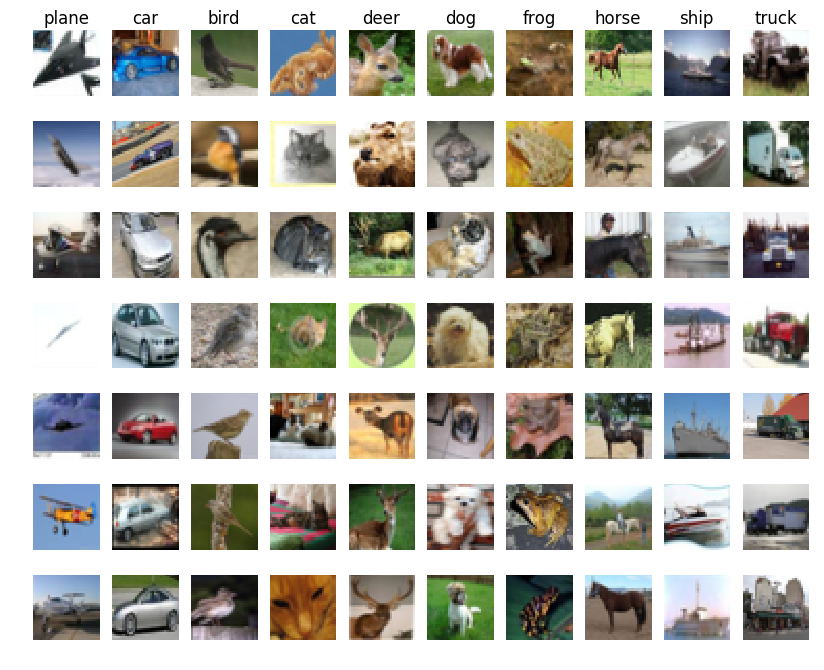
\includegraphics[width = 0.6\textwidth]{images/cifar10}
    \caption{Sample grid of images from the CIFAR10 dataset. Each one of the 32 $\times$ 32 image is labeled with one of the ten classes of objects: \textit{plane, car, bird, cat, deer, dog, frog, horse, ship, truck}.}
    \label{fig:cf10}
\end{figure}

An interesting mention in this regards should be made about \textit{semi-supervised} learning, which is typically used in bio-medical applications. This learning technique combines a large quantity of unlabeled data during training with a limited number of pre-labeled ezample. The blend between data can produce considerable improvement in learning accuracy, and leading to better results respect to pure unsupervised techniques. The typical situation of usage of this technique is when the acquisition of labeled data requires a highly trained human agent (as an anatomo-pathologist) or a complex physical experiment. The actual cost of building entire and suitable fully labeled training sets in these situations would be unbearable, and semi-supervised learnign comes in great practical help.

A good example of supervised problems tough is the classification of images. Let's assume we have a whole dataset of pictures of different objects (as cats, dogs, cars, etc.) like the CIFAR10 \cite{cifar10} dataset. This famous dataset is made of over 60$K$ labeled colored images 32$\times$32 divided into 10 categories of objects as shown in Figure \ref{fig:cf10}. We could be interested in the creation of a NN able to assign at every image its belonging class. This NN could be arbitrarily complex but it certainly will take as input a 32$\times$32$\times$3 RGB image and the output will be the predicted class. A typical output for this problem would be a probability distribution over all the 10 classes like:

\begin{align}
    \vec p & = (p_1, p_2, \dots, p_{10}), \\
    &\sum_{i=1}^{10} p_i = 1,
\end{align}
and it should be compared with the true label, that is represented just as a binary sequence $\vec t$ with the bit correspondent to the belonging class set as 1, and all the others value set to 0:

\begin{equation}
    \vec t = (0,0,\dots, 1, \dots,0,0).
\end{equation}

Every time an image is given to the model an estimate of the output is produced. Thus, we need to measure the \textit{distance} between that prediction and the true value, to quantify the error made by the algorithm and try to improve the model's predictive power. The functions used for this purpose are called loss functions. The most common choice is the Mean Squared Error (MSE) function that is simply the averaged $L^2$ norm of the difference vector between $\vec p$ and $\vec t$:

\begin{equation}
    MSE = \frac{1}{n} \sum_{i=0}^{n} (t_i - p_i)^2.
    \label{eq:MSE}
\end{equation}

Let's say the NNunder training has $L$ consecutive layers, each one with its activation function $f^k$ and its weights vector $\vec w^k$, hence the prediction vector $\vec p$ could be seen as the result of the concesutive, nested, application through all the layers:

\begin{equation}
    \vec p = f^L(\vec w^L \cdot (f^{L-1}(\vec w^{L-1} \cdot ... \cdot f^1(\vec w^1 \cdot \vec x)))).
    \label{eq:neste_layers}
\end{equation}

From both equations \ref{eq:MSE} and \ref{eq:neste_layers} it is clear that the loss function could be seen as a function of all the weights vectors of every layer of the network. So if we want to reduce the distance between the NN prediction and the true value we need to modify those weights to minimize the loss function. The most established algorithm to do so for a supervised task in a feed-forward network is the so-called \textit{error back-propagation}. The back-propagation method is an iterative technique that works essentially computing the gradient of the loss function with respect to the weights using the derivative chain rule and updating by a small amount the value of each parameter to lower the overall loss function at each step. Each weight is  \textit{moved} counter-gradient, and summing all the contribution to every parameter the loss function approaches its minimum. In equation \ref{eq:weight_update} is represented the variation applied to the $j^{th}$ weight in the $i^{th}$ layer in a single step of the method:

\begin{equation}
    \Delta w_{ij} = - \eta \frac{\partial E}{\partial w_{ij}},
    \label{eq:weight_update}
\end{equation}
where $E$ is the error function, and $\eta$ is the \textit{learning coefficient}, that modulate the effect of learning through all the training process. This iterative procedure is applied completely to each image in the training set several times, each time the whole dataset is reprocessed is called an \textit{epoch}. The great majority of the dataset is exploited in the training phase to keep running this trial and error process and just a small portion is left out (typically 10\% of the data) for a final performance test.

The loss function shall inevitably be differentiable, and its behavior heavily influences the success of the training. If the loss function presents a gradient landscape rich of local minima the gradient descent process would probably get stuck in one of them. More sophisticated algorithms capable of avoiding this issue have been devised, with the insertion of some degree of randomness in them, as the Stochastic Gradient Descent algorithm, or the wide used \textit{Adam} optimizer \cite{1412.6980}.

While Error-Back Propagation is the most established standard in DL applications, it suffers from some problems. The most common one is the so-called vanishing or exploding gradient issue, which is due to the iterative chain derivation through all the nested level of composition of the function. Withouth a careful choice of the right activation function and the tuning of the learning hyper-parameters it is very easy to bump into this pitfall. Furthermore the heavy use of derivation rises the inability to handle non-differentiable components and hinders the possibility of parallel computation. However, there are many alternative approaches to network learning beside EBP. The Minimization with Auxiliary Variables (MAV) method builds upon previously proposed methods that break the nested objective into easier-to-solve local subproblems via inserting auxiliary variables corresponding to activations in each layer. Such method avoids gradient chain computation and the potential issues associated with it \cite{1806.09077}. A further alternative approach to train the network is the Local Error Signals (LES), which is based on layer-wise loss functions. In \cite{1901.06656}, the authors demonstrate that layer-wise training can approach the state-of-the-art on a variety of image datasets. We use single-layer sub-networks and two different supervised loss functions to generate local error signals for the hidden layers, and we show that the combination of these losses helps with optimization in the context of local learning.

The training phase is the pulsing heart of a DL model development and it could take even weeks on top-level computers for the most complicated networks. In fact, one of the great limits to the complexity of a network during the designing phase is exactly the available computational power. There are many more further technical details necessary for proper training, the adjustment of which can heavily impact the quality of the algorithm. However, after the training phase, we need to test the performance of the NN. This is usually done running the trained algorithm on never seen before inputs (the test dataset) and comparing the prediction with the ground-truth value. A good way to evaluate the quality of the results is to use the same function used as the loss function during the training, but there is no technical restriction to the choice of this quality metric. The average score on the whole test set is then used as a numerical score for the network, and it allows straightforward comparison with other models' performances, trained for the same task. All this training procedure is coherently customized to every different application, depending on which the problem is posed as supervised or not and depending on the more or less complex network's architecture. The leitmotif is always finding a suitable loss function that quantifies how well the network does what it has been designed to do and trying to minimize it, operating on the parameters that define the network structure.
